\section{Objectives}

Complete the nine dynamic-logic experiments on handout PDF pages 99--106: charge sharing, explicit and parasitic coupling, leakage, three remedies, and power comparison at 500 MHz.

\section{Handout requirements and test mapping}

\begin{center}
\small
\setlength{\tabcolsep}{4pt}
\begin{tabular}{p{.42\linewidth}p{.29\linewidth}p{.18\linewidth}}
\toprule
Requirement & Deck prefix and conditions & Status \\
\midrule
Step 1: NAND charge sharing & 01; A rises, B=0 & Measured \\
Steps 2--4: CC sweep, inversion, move to output & 02; 5--50 fF & Transition bracket observed \\
Steps 5--6: upper/lower NAND gate coupling & 03; intrinsic coupling & Measured \\
Step 7: leakage during long evaluation & 04; 20 us, 25/115 C & Measured \\
Step 8: always-on/feedback keeper & 04/05/06; 500 MHz & Retention, sharing, power \\
Step 9: internal-node precharge & 04/05 & Sharing/leakage separated \\
\bottomrule
\end{tabular}
\end{center}

\section{Circuit and derivation}

The dynamic NAND precharges at low clock and evaluates at high clock. An explicit 5 fF is placed at both output and internal stack nodes for reproducibility, in addition to MOS parasitics. A lossless sharing estimate is $V_f=(C_YV_{Y0}+C_XV_{X0})/(C_Y+C_X)$, but threshold, body effect, initial levels, and feedthrough prevent exact agreement with an ideal equal-capacitor result.

A rapid aggressor transition approximately induces $\Delta V_Y\simeq C_C\Delta V_A/(C_Y+C_C)$. A driven inverter output has a restoring low-impedance path, whereas a floating dynamic node can retain erroneous charge. Keepers use weak PMOS devices with $W/L=0.3/2\,\mu\mathrm m$; the internal precharge PMOS uses $0.6/0.25\,\mu\mathrm m$.

\section{Simulation setup and interpretation}

The supplied encrypted MOS model is evaluated at a baseline supply of 1.0 V and 25\,$^\circ$C. The 1.0 V value is a teaching condition, not a verified voltage rating. These results do not reproduce the handout's original process or supply conditions. Unless stated in the deck, $W_n/W_p/L=0.6/1.8/0.25\,\mu\mathrm m$, bulks are tied to their corresponding rails, and output load is 5 fF. Transmission-gate and weak-feedback dimensions are specified explicitly in each deck.

PrimeSim HSPICE S-2021.09 win64 was used with \texttt{RUNLVL=6}, \texttt{ACCURATE}, and \texttt{WARNLIMIT=100}. Every baseline and \texttt{.alter} analysis concluded without errors or failed measurements. The simulator still reports suppressed warnings associated with encrypted blocks; this does not establish that the model is warning-free or that those warnings are harmless. The \texttt{.tran} print interval is not a fixed integration step: the solver uses adaptive timesteps. A finite sweep is not a complete process qualification.

Unless stated otherwise, the declared functional diagnostic uses $V\leq0.2$ V for low and $V\geq0.8$ V for high. These are report-level interpretation thresholds, not numerical handout requirements or extracted receiver noise margins. Correct samples do not exclude glitches between samples. Figures are redrawn from actual simulation data; \texttt{results/} contains per-case waveforms, measurements, and derived comparison CSV files.

Public decks omit model loading paths; model configuration is added only to local execution copies. The model itself is not distributed. The first two filename digits identify the deck numbers used below. Every deck is standalone.

\section{Results}

In the basic sharing case without an output inverter, Y falls from 1.172805 to 0.701010 V, a 0.471795 V drop, while internal X reaches 0.622395 V. The initial value above 1 V is clock feedthrough, not a higher supply. Remedy comparisons use a separate set with matched inverter loading; their baseline droop differs and must not be mixed with this unloaded result.

\begin{figure}[htbp]
\centering
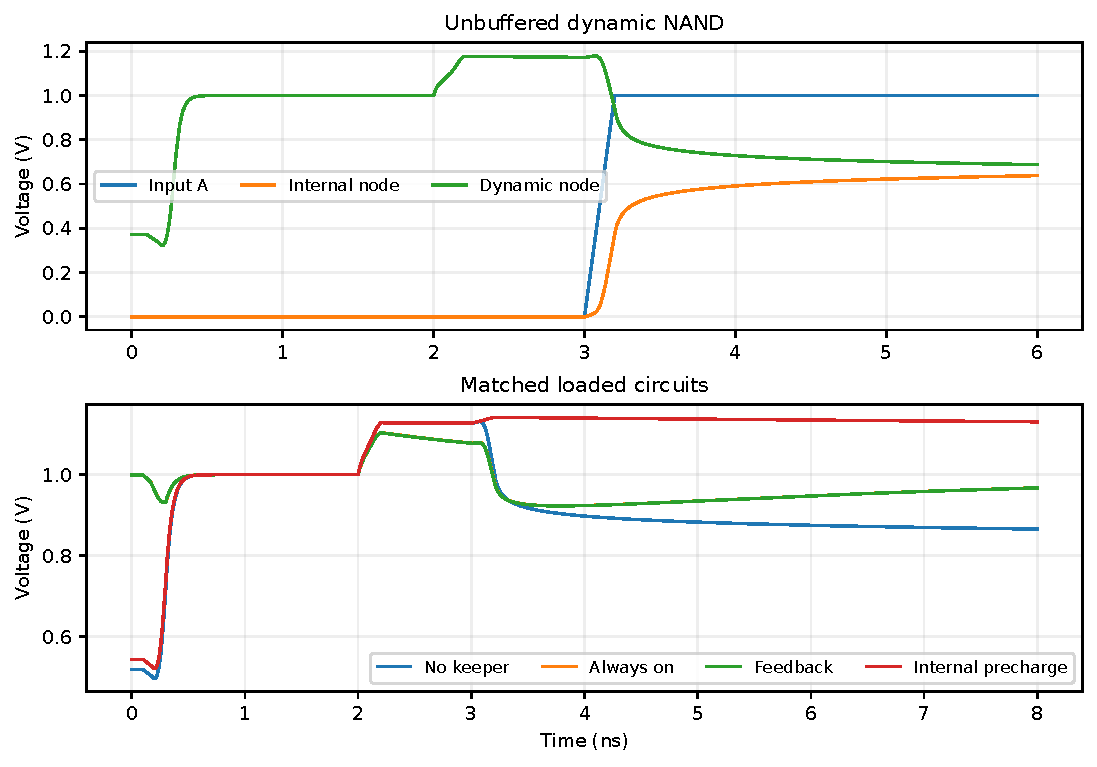
\includegraphics[width=.96\linewidth]{figures/charge_sharing.pdf}
\caption{Basic sharing and the three remedies under matched loading.}
\end{figure}

\begin{center}
\small
\setlength{\tabcolsep}{4pt}
\begin{tabular}{lrrr}
\toprule
Coupling (fF) & Dynamic Y (V) & Inverter output (V) & Direct-output minimum (V) \\
\midrule
5 & 0.8277 & 0.0000 & -0.2632 \\
10 & 0.6555 & 0.0026 & -0.4427 \\
15 & 0.5511 & 0.0221 & -0.5547 \\
20 & 0.4845 & 0.2850 & -0.6161 \\
30 & 0.4027 & 0.9760 & -0.6562 \\
50 & 0.2859 & 0.9985 & -0.6843 \\
\bottomrule
\end{tabular}
\end{center}

At CC=20 fF, the following inverter output is 0.284995 V, inside this report's conservative indeterminate region. At 30 fF it is 0.976020 V, a clear erroneous high. Using 0.5 V as a receiver decision level brackets the transition between 20 and 30 fF. The same 30 fF coupled directly to the inverter output briefly drives it to -0.656 V, but it recovers to approximately 0 V by 6 ns. Recovery within this window does not mean the spike is harmless to every receiver.

\begin{figure}[htbp]
\centering
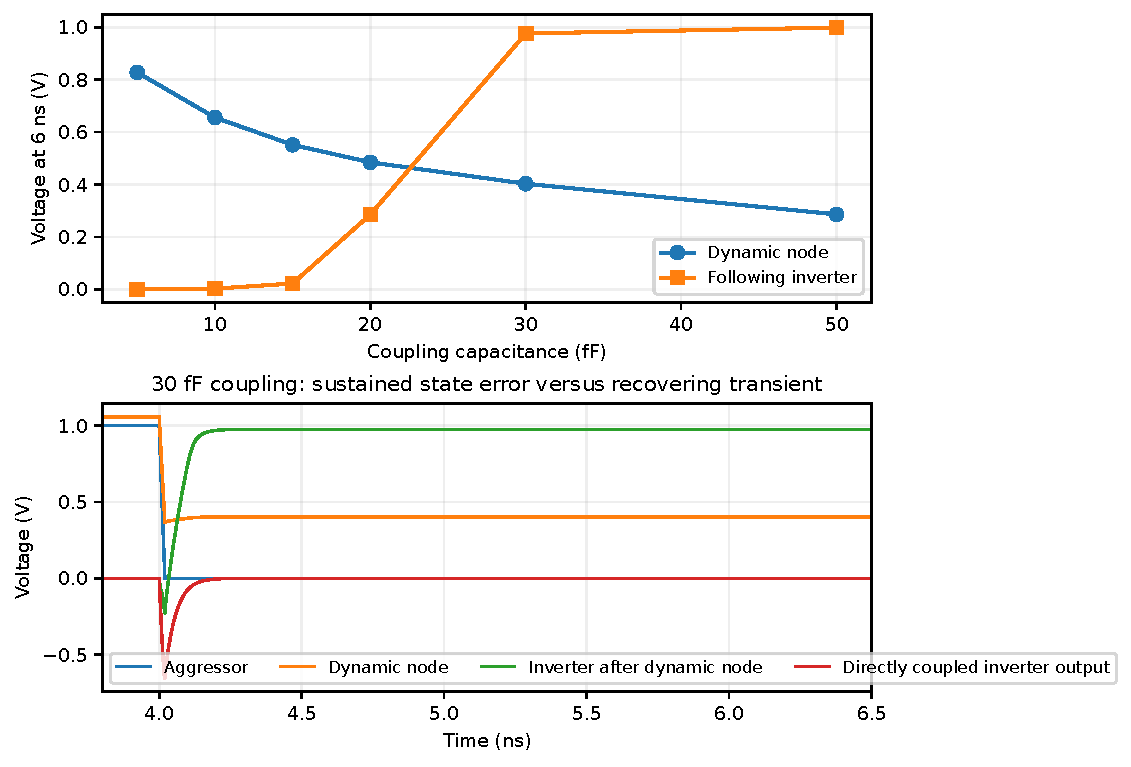
\includegraphics[width=.96\linewidth]{figures/coupling.pdf}
\caption{CC sweep and representative 30 fF waveforms, distinguishing sustained error from a recovering spike.}
\end{figure}

\begin{center}
\small
\setlength{\tabcolsep}{4pt}
\begin{tabular}{lrrr}
\toprule
NAND gate position & Before (V) & After (V) & Drop (V) \\
\midrule
upper & 1.13912 & 0.94524 & 0.19388 \\
lower & 1.12564 & 1.07639 & 0.04925 \\
\bottomrule
\end{tabular}
\end{center}

With no added CC and only device parasitics, coupling at the upper NMOS gate produces a 0.193876 V Y drop, versus 0.049251 V at the lower gate. This supports the role of gate/source/drain location and intermediate-node shielding: logically equivalent input pins need not have equal analog sensitivity.

\begin{figure}[htbp]
\centering
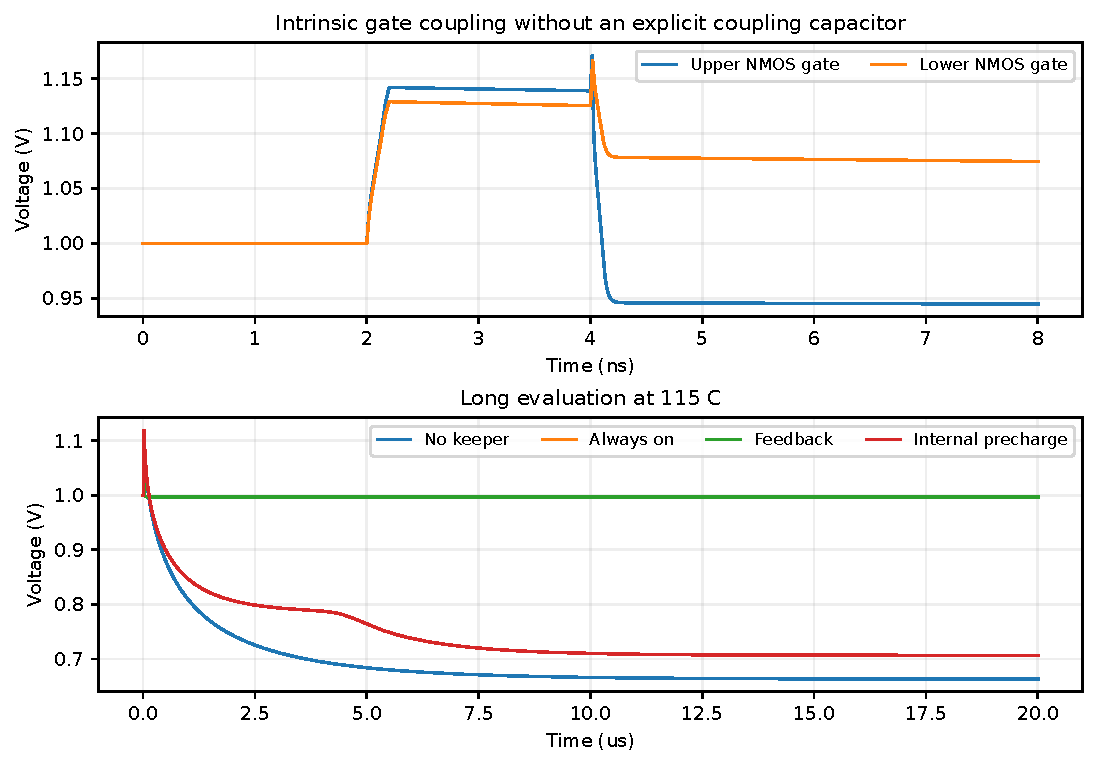
\includegraphics[width=.96\linewidth]{figures/coupling_and_retention.pdf}
\caption{Upper: intrinsic parasitic coupling. Lower: 20 us retention at 115 C.}
\end{figure}

\begin{center}
\small
\setlength{\tabcolsep}{4pt}
\begin{tabular}{lrrr}
\toprule
Remedy & Sharing drop (V) & Final at 25 C (V) & Final at 115 C (V) \\
\midrule
None & 0.24463 & 0.53783 & 0.66294 \\
Always on & 0.14851 & 0.99896 & 0.99702 \\
Feedback & 0.14830 & 0.99896 & 0.99702 \\
Internal precharge & -0.01016 & 0.58577 & 0.70663 \\
\bottomrule
\end{tabular}
\end{center}

Always-on and feedback keepers maintain long-hold levels near 0.997--0.999 V. Internal precharge suppresses sharing but does not continuously replenish charge during evaluation. The uncorrected final level is higher at 115 C than at 25 C, showing that net current depends on multiple paths in this model and bias condition. It must not be rewritten as necessarily faster decay at higher temperature. A complete inverter logic flip was not observed within 20 us in this leakage test.

\begin{center}
\small
\setlength{\tabcolsep}{4pt}
\begin{tabular}{lrrrr}
\toprule
Freq. (MHz) & Always power (uW) & Feedback power (uW) & Always eval. (uA) & Feedback eval. (uA) \\
\midrule
500 & 16.1263 & 16.5449 & 9.9347 & 8.2381 \\
50 & 2.4854 & 1.6582 & 1.8482 & 0.6664 \\
\bottomrule
\end{tabular}
\end{center}

\begin{figure}[htbp]
\centering
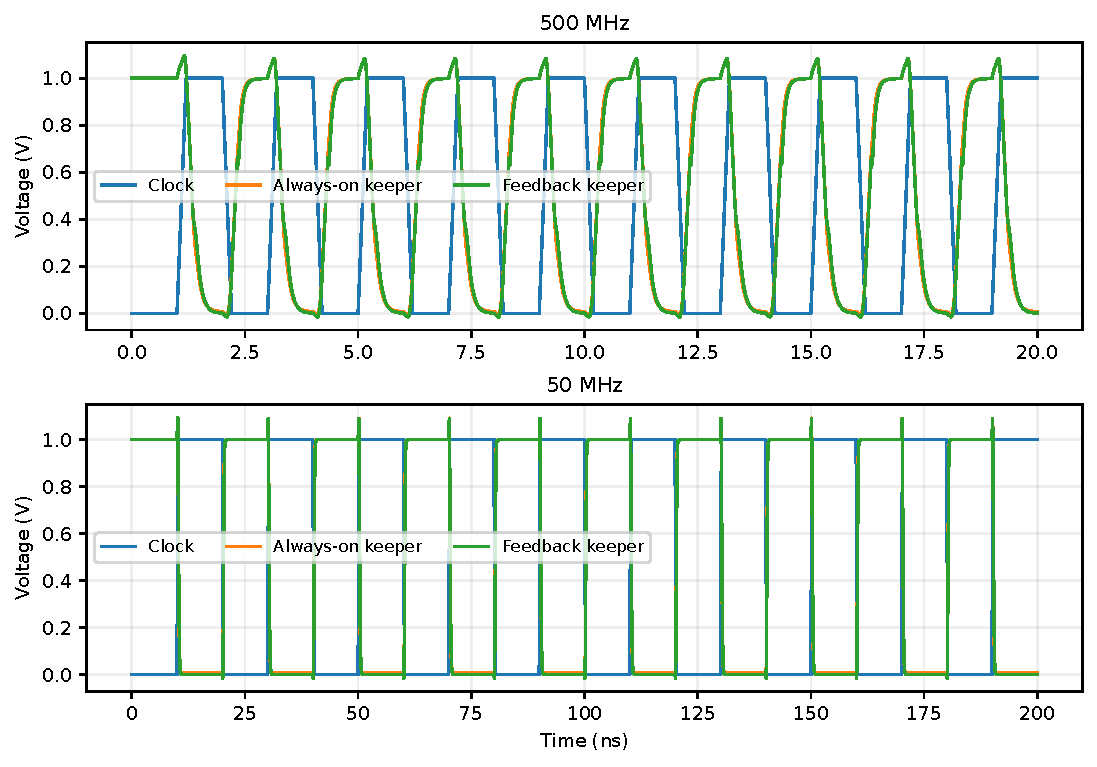
\includegraphics[width=.96\linewidth]{figures/keeper_power.pdf}
\caption{The required 500 MHz test is retained; 50 MHz is added as a more fully settled comparison.}
\end{figure}

\section{Discussion, differences, and unverified scope}

At 500 MHz, feedback average power is 16.5449\,$\mu$W, slightly above 16.1263\,$\mu$W for always-on. Feedback must not be declared universally lower-power. Its evaluation current is lower, but cycle-average power also includes dynamic charging, delay, and switching contention. At 50 MHz, feedback average power falls to 1.6582\,$\mu$W versus 2.4854\,$\mu$W for always-on. Power is averaged over $2T$--$10T$ and evaluation current over $8.7T$--$8.9T$. All nine observations have corresponding tests; qualitative handout explanations are not converted into invented numerical pass/fail requirements.
